\documentclass{standalone}

\usepackage{tikz}
\usepackage{standalone}
\usetikzlibrary{calc}

\begin{document}

    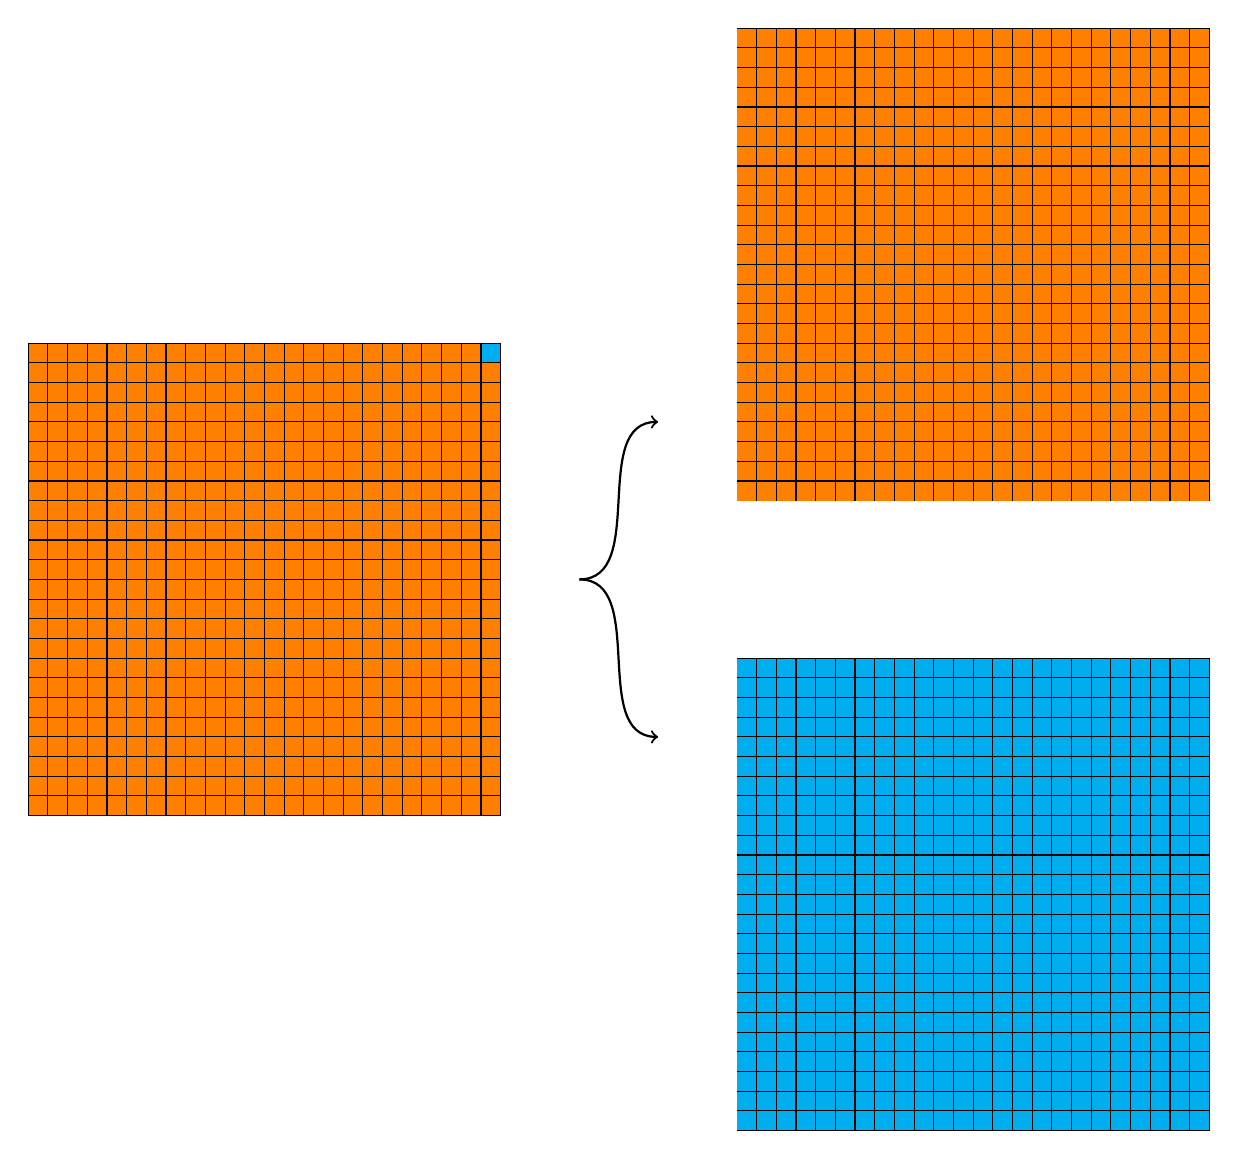
\begin{tikzpicture}

        \fill[orange] (0, 0) rectangle (6, 6);
        \fill[cyan] (5.75,5.75) rectangle (6,6);
        \draw[step=0.25cm, black] (0, 0) grid (6, 6);

        \fill[cyan] (9,-4) rectangle (15,2);
        \draw[step=0.25cm, black] (9,-4) grid (15,2);

        \fill[orange] (9,4) rectangle (15,10);
        \draw[step=0.25cm, black] (9, 4) grid (15, 10);

        \draw[step=0.25cm, black] (0,0) grid (6,6);

        \draw (7, 3) edge[out=0, in=-180, ->, thick] (8, 5);
        \draw (7, 3) edge[out=0, in=-180, ->, thick] (8, 1);

        % \draw (16, 7) edge[out=0, in=-180, ->, thick] (17, 7);
        % \draw (16, -1) edge[out=0, in=-180, ->, thick] (17, -1);

    \end{tikzpicture}

\end{document}